% Final manuscript: completed DeepSeek/Gemini campaigns and domain case study.
% Build from the repository root: latexmk -pdf main.tex
\documentclass[10pt,conference]{IEEEtran}
\usepackage[T1]{fontenc}
\usepackage{amsmath,amssymb}
\usepackage{booktabs,array,tabularx}
\usepackage{graphicx,xcolor}
\usepackage[most]{tcolorbox}
\definecolor{rqback}{HTML}{F2F4F7}
\definecolor{rqframe}{HTML}{4A5568}
\usepackage{xurl}
\usepackage{cite}
\usepackage[hidelinks]{hyperref}
\newcommand{\tracer}{\textsc{Tracer}}
\newcommand{\code}[1]{\texttt{\detokenize{#1}}}
\newcommand{\rqfinding}[2]{%
  \begin{tcolorbox}[
    colback=rqback, colframe=rqframe,
    boxrule=0.4pt, leftrule=3.5pt, arc=1.5pt,
    left=6pt, right=6pt, top=5pt, bottom=5pt,
    fontupper=\small
  ]
  \textbf{#1.} #2
  \end{tcolorbox}%
}
\emergencystretch=1em
\title{Securing Agent-Generated Code Through Development History}
\author{
\IEEEauthorblockN{Prateek Rajput\IEEEauthorrefmark{1},
Shahzeb Khan\IEEEauthorrefmark{2},
Jacques Klein\IEEEauthorrefmark{1}, and
Tegawend\'e F. Bissyand\'e\IEEEauthorrefmark{1}}
\IEEEauthorblockA{\IEEEauthorrefmark{1}University of Luxembourg, Luxembourg\\
\{prateek.rajput, jacques.klein, tegawende.bissyande\}@uni.lu}
\IEEEauthorblockA{\IEEEauthorrefmark{2}Nostrum Biodiscovery S.L., Barcelona, Spain\\
shahzeb.khan@nostrumbiodiscovery.com
}
}

\begin{document}
\bstctlcite{IEEEexample:BSTcontrol}
\maketitle
\begin{abstract}
Agentic software development makes it possible to capture the process of code creation, moving beyond static comments and commit messages to preserve edits, tool interactions, and recorded ReAct-style reasoning behind implementation decisions. We present \tracer{} (Trace-based Runtime Analysis for Continuous Evolution and Release), a provenance-aware workflow that links task descriptions and recorded agent rationale to the evolution of code and its constituent symbols. We ask whether combining these reasoning traces with code evolution helps investigators understand implementation assumptions and better diagnose and fix security flaws. \tracer{} preserves diagnostic evidence, repair rationale, and associated executable boundary checks alongside each repair, providing persistent context for future updates, refactors, and feature additions. Across 3,096 repair runs on the SusVibes benchmark, \tracer{}'s change-informed planning covers reference-vulnerable symbols in 94.6\% of attempts, compared with 13.4\% for stock SAST locations. The rationale-enabled configuration achieves the highest verified security pass rates among the evaluated configurations with both investigators, while a stage-level analysis exposes where remaining candidates are lost during diagnosis and validation. Extending \tracer{} to real-world structural-biology repositories, we verify five component repairs and evaluate subsequent feature evolution under silent-fix conditions, where pairing persistent repair memory with a boundary gate and one feedback retry improves joint feature-and-security-check success from 3/5 to 5/5.
\end{abstract}
\begin{IEEEkeywords}
Agentic Software Engineering, Vulnerability Repair, Provenance and Reasoning Traces, Silent Security Fixes, Continuous Software Evolution, Static and Dynamic Analysis.
\end{IEEEkeywords}

\begin{figure*}[t]
\centering
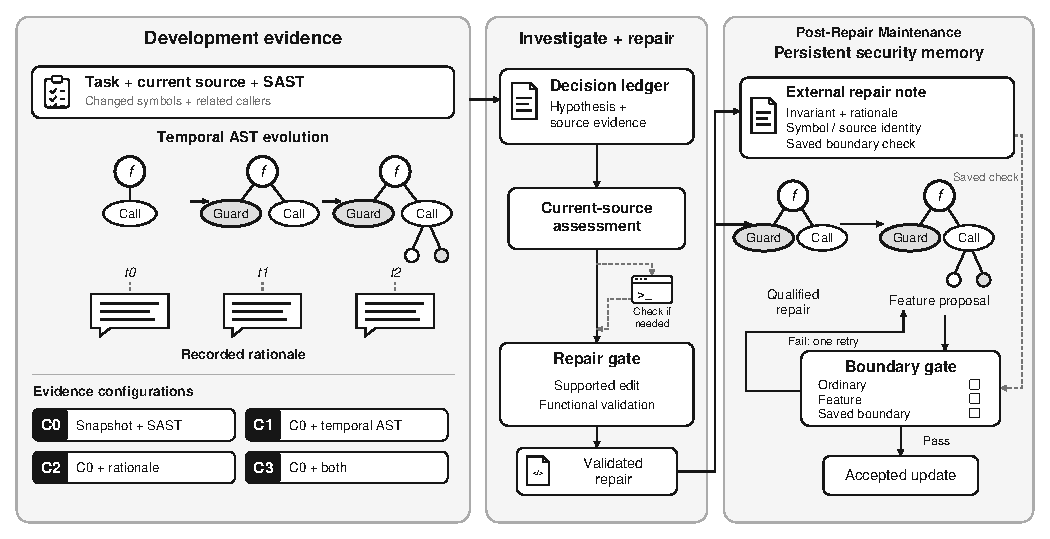
\includegraphics[width=\textwidth]{figures/tracer_security_overview.pdf}
\caption{\tracer{} links symbol-level development evidence to guarded security repair, then preserves repair invariants and executable checks for subsequent feature evolution. C0--C3 vary the evidence available during investigation.}
\label{fig:architecture}
\end{figure*}

\section{Introduction}
Autonomous coding agents can navigate repositories, edit source files, and execute test suites through interfaces such as SWE-agent~\cite{sweagent}, while agent-based repair systems extend this tool-driven workflow to debugging~\cite{repairagent}. For engineering teams adopting these systems, security remains a critical review obligation. Empirical studies of generated code and coding-assistant use document security weaknesses~\cite{asleep,perry,copilotweaknesses}. A patch can satisfy functional tests while leaving an unsafe input boundary, incomplete validation, or a violated API contract. SusVibes makes this gap explicit by evaluating functionality and security separately on repository-level tasks~\cite{susvibes,susvibesartifact}. Teams accepting working, agent-generated changes therefore need to uncover and repair omitted security conditions without breaking the requested functionality.

Existing software engineering defenses provide several starting points. Static application security testing (SAST) tools such as CodeQL~\cite{codeql} and Semgrep~\cite{semgrep} supply reproducible rules, source locations, and flow evidence. Industrial deployments and developer studies emphasize integrating actionable diagnostics into code review~\cite{johnson,googleanalysis,infer}. LLM-assisted taint and dataflow analysis~\cite{iris,llmdfa,repoaudit}, analyzer-guided repair~\cite{inferfix}, and program-analysis-guided proof-of-concept generation~\cite{pagent} further connect model judgments to source and execution evidence. These techniques help examine the implementation under review, but current-source findings alone do not explain why a coding agent omitted a guard or what it assumed about upstream inputs. When scanner locations also miss the relevant changed symbols, an investigator must first establish where to look and then reconstruct the missing security condition.

Agentic development offers the recorded process of code creation as an additional source of evidence. A trajectory can preserve intermediate edits, tool interactions, and interleaved ReAct-style explanations~\cite{react}, extending the evidence available from a final diff and commit message. Fine-grained AST differencing makes structural changes explicit~\cite{gumtree}, while recorded rationale supplies statements about input trust, callers, and library behavior. Together, these channels can expose a removed guard, an asymmetry between sibling functions, or a mismatch between an agent's stated assumption and its implementation. We treat explanations as hypotheses to check against current source, since generated rationale need not faithfully reveal internal reasoning~\cite{turpin,lanham}. The opportunity is to connect the history of a change to the present security contract that a repair must satisfy.

Repair is also a maintenance problem. Work on silent vulnerability fixes shows that security-relevant changes can lack an explicit security designation~\cite{colefunda}, and subsequent edits can undo an earlier repair, as explored in security-regression studies~\cite{undoingfix}. A later refactor or feature addition may preserve the requested behavior while losing a condition whose purpose is no longer apparent. The same provenance collected during investigation can carry that purpose forward. The diagnostic evidence, enforced invariant, and independently owned executable boundary check can remain linked to the repaired symbol. A maintenance workflow can then test subsequent changes against the saved contract and return concrete feedback when they violate it.

We present \tracer{} (\emph{Trace-based Runtime Analysis for Continuous Evolution and Release}), a provenance-aware security investigation, repair, and maintenance workflow packaged as a lightweight, portable skill for integration with coding agents and continuous-integration pipelines. Given a bounded Git range or a compatible agent trajectory, \tracer{} performs change-informed symbol planning, keeps typed AST evolution separate from recorded rationale, grounds repair decisions in current-source assessment and conditional runtime checks, and emits persistent repair notes that can be coupled with executable boundary gates. Across 3,096 SusVibes repair runs spanning seven coding generators and two security investigators, its planner includes reference-vulnerable symbols in 94.6\% of attempts, compared with 13.4\% primary SAST symbol overlap. The rationale-enabled configuration achieves the highest verified security pass counts with both investigators. Combining both history channels does not improve on it. A complementary study of structural-biology software~\cite{rfdiffusion,proteinmpnn,haddock3,dockq,vina,foldseek} verifies five component repairs and tests their subsequent feature evolution. Persistent memory with a one-retry boundary gate achieves joint feature-and-boundary success in 5/5 cases, compared with 3/5 for unguarded continuation.

The paper makes three contributions.
\begin{itemize}
    \item \textbf{A provenance-aware architecture and portable skill.} \tracer{} connects change-informed planning, separate AST-evolution and rationale channels, guarded static/dynamic investigation, and persistent repair memory in a workflow that can accompany an agent-generated change through later maintenance.
    \item \textbf{A multi-investigator evaluation.} The SusVibes study compares four context bundles across seven coding generators and two investigators, measuring review coverage, verified security outcomes, and functional preservation. The structural-biology study evaluates the maintenance stage under silent-fix feature evolution.
    \item \textbf{A stage-level funnel and failure taxonomy.} A seven-version engineering progression and a full-cohort investigation funnel identify losses during diagnosis, validation scheduling, patch retention, and semantic repair, providing concrete design lessons for agentic review systems.
\end{itemize}

\section{Background and Motivation}
\label{sec:motivation}
\subsection{Industry Relevance and Code Archaeology}
When an agent-generated pull request works, an industrial reviewer must still determine which implementation assumptions deserve scrutiny and which security conditions must survive later maintenance. CodeQL and Semgrep can report locations and flows in the final snapshot~\cite{codeql,semgrep}, but the reviewer must connect those findings to the submitted change, affected callers, and the intended contract. We call this reconstruction \emph{code archaeology}. It recovers the context behind the current implementation from the evidence left available. Industrial static-analysis studies emphasize actionable diagnostics, developer trust, and integration into existing review workflows~\cite{johnson,googleanalysis,infer}. Preserving the development trace can supply context for that review, especially when the final diff omits an intermediate decision or correction.

For scientific-software teams such as Nostrum Biodiscovery, checkpoint loading, structure parsing, archive extraction, and output-path handling are concrete interfaces where compatibility requests can invalidate earlier assumptions. A useful workflow must investigate these boundaries while preserving the requested scientific functionality, then retain the repair's purpose for the next change. Connecting review evidence to reusable checks fits secure-development practices for code review, testing, and retaining vulnerability knowledge~\cite{ssdf}. Our domain study examines these component-level obligations. Production effectiveness remains to be evaluated.

\subsection{Tracking Structural Evolution Within a Bounded Context}
Making history available is not equivalent to making it usable. Source lines shift, definitions are added or renamed, and refactoring changes how code is divided among functions and classes. Intermediate fragments may not parse. A temporal representation therefore cannot assume that node names or line positions remain stable across versions. A line-based \code{git diff} records textual changes, but does not itself establish which function-level contract changed. Retaining every full AST and cross-version relation also expands the context with repeated or irrelevant structure. Fine-grained AST matching through GumTree~\cite{gumtree,gumtree3}, together with function-change representations such as CoLeFunDa's~\cite{colefunda}, motivates a focused representation that maps observed changes to symbols, summarizes their structural edits, and preserves explicit gaps where continuity cannot be established.

\subsection{Task Intent and Recorded Reasoning}
Static analysis and AST differencing answer complementary questions about reported flows and structural changes, but neither alone supplies the requested behavior or every domain-specific assumption. Code can execute successfully while mishandling an input representation, trusting a caller without justification, or implementing only part of the task's contract. ReAct-style trajectories interleave explanations with actions~\cite{react}, allowing the task description, stated assumptions, and observed edits to be examined together. These recorded explanations are auditable claims, not guaranteed accounts of internal chain-of-thought~\cite{turpin,lanham}. A statement that an input is already validated, for example, creates a concrete obligation to inspect the relevant validator and its callers.

Our motivating cases come from repository tasks in SusVibes~\cite{susvibes,susvibesartifact}. In Python-RSA,\footnote{\url{https://github.com/sybrenstuvel/python-rsa}} comparing \code{decrypt} and \code{verify} exposes an asymmetric encoded-input-length guard. LangChain\footnote{\url{https://github.com/langchain-ai/langchain}} similarly illustrates an incomplete origin condition that checks network location but omits scheme equality. Wagtail CMS\footnote{\url{https://github.com/wagtail/wagtail}} shows the danger of repairing an intermediate label without inspecting downstream rendering. An early candidate introduces double-escaping. In Django,\footnote{\url{https://github.com/django/django}} recorded rationale favors character-reference conversion in \code{strip_tags}, while its tested contract requires preserving relevant text representations. A partial handler repair still fails. These cases motivate both discovering missing invariants and checking a proposed repair at the correct boundary.

\section{TRACER Architecture and Portable Skill}
\label{sec:architecture}

\subsection{Symbol-Level Tracking and Snapshot SAST (C0)}
The evaluated Python pipeline builds a symbol-level index using the standard-library \code{ast.parse} parser~\cite{pythonast} and a custom AST visitor. For each parsed snapshot, the index records functions, asynchronous functions, methods, and classes by repository path, qualified name, and definition span. The history adapter also records structural hashes. Rather than using diff lines as the review unit, the planner maps submitted patch hunks and deletion anchors to their enclosing current symbols, excludes test and documentation paths, and records module-level or unavailable mappings when needed. It links guards, candidate in-file callers, and related changed symbols, while attributing Semgrep and CodeQL locations and flow evidence to their originating scanners~\cite{semgrep,codeql}. Local call-name matches are syntactic review hints, not resolved dataflow. This channel defines C0 as a change-informed snapshot review that scopes investigation beyond scanner locations, but still requires archaeology to explain how and why the current symbol was written.

\subsection{Temporal AST Evolution via GumTree (C1)}
C1 adds the observed structural evolution of selected symbols. \tracer{} parses available before/after source pairs into typed Python ASTs and computes edit scripts with GumTree 3.0.0~\cite{gumtree,gumtree3}. It filters operations to the target symbols, retains guards and calls inside parent-subtree additions, normalizes recoverable fragment indentation, and bounds operations, symbol summaries, and delivered characters. The resulting hints describe changes without passing every historical snapshot to the investigator. Cutoff-bounded Git ancestry and recorded agent edits retain separate provenance. Path/name associations and unique fragment anchors link evidence to current symbols. Continuity gaps, parse failures, and truncation remain explicit rather than implying complete identity tracking through arbitrary renames or refactors.

\subsection{Symbol-Linked Reasoning Traces (C2 and C3)}
The task description is shared context for every configuration. C2 additionally retrieves original ReAct-style development prose~\cite{react}, excluding fenced code so explanations remain separate from source changes. The extractor links excerpts through recorded action paths, symbol mentions, and uniquely matched edit fragments, retaining event IDs, offsets, and source hashes. A file association remains distinguishable from a current-symbol anchor. When an excerpt informs a hypothesis, its quotation, testable assumption, and verification plan are stored with that hypothesis's target symbol in the decision ledger. The investigator records whether current evidence supports, contradicts, or leaves the assumption unresolved, since rationale is not authoritative evidence of behavior~\cite{turpin,lanham}. C3 combines these rationale links with C1's temporal AST evidence and divergence cues. Rationale retrieval remains available even when an old AST cannot be reconstructed.

\subsection{Decision Ledger, Repair Gate, and Portable Skill}
The investigator records a hypothesis's target symbol, input boundary, and alleged violated property in a structured decision ledger, serialized in \code{edit_note.json}. It grounds assessments in quotations from the current source and, when evidence remains inconclusive, bounded Python checks following PAGENT's analysis-guided testing pattern~\cite{pagent}. Checks record the source version, target reachability, ordinary-input behavior, and boundary observations. The repair gate requires a supported defect, review of relevant downstream consumers, and validation of the candidate against public functional tests. Assessments and checks must apply to the current candidate. The note preserves their evidence links alongside patch, source, and trajectory identities.

For Stage~4 maintenance, a qualified repair note additionally binds the security invariant to the exact repaired-symbol hash and an independently owned executable boundary check. Subsequent feature proposals must satisfy ordinary, feature, and saved boundary checks. The continuation gate returns failure feedback for a bounded retry or retains the qualified starting code, recording acceptance and fallback separately.

The portable \code{tracer-security} skill\footnote{\url{https://github.com/pkrajput/TRACER_skill}} packages this symbol-tracking and ledger workflow for a host coding agent. Local helpers consume a bounded Git history or compatible recorded trajectory and produce review evidence using the available scanner and history adapters. The host supplies its editing and test interface, while a CI pipeline can run the saved checks on later changes. This separation supports adoption without depending on the SusVibes runner or its hidden evaluation tests.

\section{Experimental Design and Reproducibility}
\label{sec:design}
\subsection{Research Questions}
We structure the evaluation around five research questions that follow an agent-generated change from initial localization to subsequent maintenance. These are retrospective reporting questions for the completed experiments.

\noindent\textbf{RQ1 (Localization Coverage).} \emph{How effectively does change-informed planning expose vulnerable symbols compared with stock SAST locations?}\par
Diagnosis requires bringing the relevant source into scope. We measure whether patch-selected symbols and their relations expose reference-relevant code beyond the locations reported by the scanners.

\smallskip
\noindent\textbf{RQ2 (End-to-End Verified Repair).} \emph{Does guarded investigation improve verified security outcomes without degrading functionality?}\par
Security interventions can break working features. We measure security conversions and functional regressions after current-source assessment, conditional runtime checks, and public functional validation.

\smallskip
\noindent\textbf{RQ3 (Provenance Channels).} \emph{How do temporal AST history, recorded rationale, and their combination affect verified repair?}\par
More context does not automatically produce better repairs. Comparing the four implemented bundles on identical attempts measures their relative contribution, with accompanying audit cues treated as part of each bundle.

\smallskip
\noindent\textbf{RQ4 (Stage-Level Bottlenecks).} \emph{Where are candidates lost between symbol localization and verified repair?}\par
Review coverage does not guarantee a successful patch. A seven-version development study and a four-stage investigation funnel distinguish diagnostic, validation, semantic, and operational losses.

\smallskip
\noindent\textbf{RQ5 (Persistent Memory Under Silent-Fix Evolution).} \emph{Can repair memory and boundary gates preserve repaired properties while subsequent feature changes succeed?}\par
Later maintenance must satisfy both the new feature request and the earlier repair contract. We test whether saved repair notes and executable checks support that joint outcome in structural-biology software under silent-fix conditions.

\subsection{Benchmark, Cohort Inventory, and Evaluation Predicates}
We use SusVibes and its released functional/security evaluator~\cite{susvibes,susvibesartifact}. An \emph{attempt} pairs a task with an archived coding-generator output, while a \emph{cell} additionally identifies the investigator and configuration. Among 1,302 archived outputs from seven generators, 472 have publisher-reported functional success, and local environment reproduction and source-integrity screening admit 387 attempts across 118 tasks (Table~\ref{tab:inventory}). Each investigator contributes 1,548 cells, giving 3,096 recorded repair runs.

\begin{table}[t]
\caption{Cohort inventory, locally verified original outcomes, and review coverage. Verif. counts terminal-complete original evaluations, with Func/Sec reported on that subset. Coverage uses all 387 admissions.}
\label{tab:inventory}
\centering\footnotesize
% Generated by paper/build_final_tables.py; FINAL_MANUSCRIPT_DATA.json
\begin{tabular}{@{}lrrrrr@{}}
\toprule
Generator & Source & Admit. & Verif. & Func & Sec \\
\midrule
Claude 4 Sonnet & 186 & 88 & 83 & 81 & 15 \\
Gemini 2.5 Pro & 186 & 29 & 24 & 24 & 6 \\
Gemini 3 Pro & 186 & 58 & 55 & 54 & 16 \\
GLM-4.7-Flash & 186 & 38 & 30 & 30 & 5 \\
GLM-5 & 186 & 100 & 98 & 98 & 17 \\
Kimi K2 & 186 & 33 & 28 & 27 & 4 \\
Qwen3-Coder-Next & 186 & 41 & 36 & 36 & 6 \\
\midrule
Total & 1302 & 387 & 354 & 350 & 69 \\
\midrule
\multicolumn{6}{@{}l}{\textit{Coverage among all 387 admitted attempts}} \\
\multicolumn{4}{@{}l}{SAST reference file} & 228 & 58.9\% \\
\multicolumn{4}{@{}l}{SAST primary reference symbol} & 52 & 13.4\% \\
\multicolumn{4}{@{}l}{SAST symbol including flow endpoints} & 63 & 16.3\% \\
\multicolumn{4}{@{}l}{Change-informed plan reference symbol} & 366 & 94.6\% \\
\bottomrule
\end{tabular}

\end{table}

FuncPass and SecPass require recognized framework-specific terminal summaries, including the benchmark's expected-failure allowances. The shared comparison contains 345 attempts with completed functional and security evaluations for the original output and all eight investigator/configuration candidates. DeepSeek additionally supports a 354-attempt four-configuration comparison. The other 42 admissions remain outside the shared comparison. A frozen task-level exposure split identifies 235 development-exposed and 110 previously protected shared attempts, with labels consistent across generators. These are conditional repair outcomes, not new benchmark-wide generator pass@1 estimates.

Hidden security tests and reference patches are used only for retrospective evaluation. Investigators receive public functional feedback. Recovery evaluates originals and candidates under the same restored environment, records exact-hash reuse, and preserves earlier completed cells and their execution revisions. Conversions, regressions, and unresolved execution remain separate. Task-cluster intervals use 5,000 percentile-bootstrap replicates with seed 12 to account for repeated generator attempts~\cite{bootstrap}.

\subsection{Investigated Configurations and Scanner Setup}
DeepSeek-V3.2 and Gemini-3.8-Flash investigate each attempt with temperature zero, a 22-turn cap, and a shared 100,000-byte message setting. DeepSeek uses OpenRouter's SiliconFlow FP8 endpoint, while Gemini uses its native endpoint with LOW thinking. Every configuration receives the functional request, patch-selected current source, scanner context, and the same guarded protocol.
\begin{itemize}
    \item \textbf{C0. Snapshot + SAST.} Change-informed current-source review with scanner findings.
    \item \textbf{C1. + Temporal AST.} C0 with observed structural code changes.
    \item \textbf{C2. + Recorded Rationale.} C0 with original development explanations.
    \item \textbf{C3. Combined.} C0 with both channels and linked divergence evidence.
\end{itemize}
C0 already receives agent-patch-selected targets. C1--C3 additionally receive deterministic completeness cues, without a cue-only control. Comparisons therefore concern implemented context bundles. Upstream Git ancestry is withheld to avoid revealing masked implementations, so measured temporal evidence comes from post-reference agent trajectories.

All configurations share Semgrep CE 1.101.0 with Python rules at commit \code{495df89c} and CodeQL 2.20.0 with Python queries 1.3.4 and the security-extended suite. Semgrep includes correctness and maintainability rules alongside security checks. Scans use source exports without hidden evaluation artifacts. Planning scopes findings to changed files and at most twelve groups, while overlap audits use the full scanner output. SAST-seeded attempts receive at least one scanner alert in their input, while unseeded attempts receive none. Task-level outcomes do not establish alert-level false-positive reduction.

\section{Empirical Results on Coverage and Repair Outcomes}
\label{sec:results}
\subsection{RQ1. Evidence Available for Review}
Stock SAST overlaps a reference file in 228/387 attempts (58.9\%), a primary reference symbol in 52/387 (13.4\%), and a symbol including flow positions in 63/387 (16.3\%). The planner includes a reference symbol in 366/387 plans (94.6\%) and its complete body in 329/387 (Table~\ref{tab:inventory}). The coverage gap also persists among the 291 publisher-SecFail attempts, where primary and flow-inclusive overlaps are 41 and 50, while plan inclusion reaches 281. Thus the broader review scope reaches implementations that fail the security tests, not only the admitted population in aggregate.

Patch selection and the functional request explain how C0 receives relevant context even when SAST is silent. Of 335 attempts without a primary reference-symbol warning, patch selection supplies a reference group in 317 and its complete body in 282, while functional requests mention the target in 307. The plan consequently supplies implementation context beyond reported warning locations. This remains a measure of review opportunity, with file-only mappings kept separate from named symbols.

\rqfinding{RQ1 Finding}{Change-informed planning includes reference-relevant symbols in 94.6\% of review plans, compared with 13.4\% primary SAST symbol overlap. Diagnosis and repair remain subsequent steps.}

\subsection{RQ2. Verified End-to-End Repair}
\begin{table*}[t]
\caption{Verified repair outcomes. F/S denotes FuncPass/SecPass. Shared panels use the same 345 attempts with complete outcomes for all eight investigator/configuration candidates. Each panel states its population.}
\label{tab:results}
\centering\footnotesize
% Frozen final outcomes. Bold marks each investigator's highest SecPass, including ties.
\renewcommand{\arraystretch}{1.12}
\begin{tabular*}{\textwidth}{@{\extracolsep{\fill}}lrrrrrr@{}}
\toprule
Population or investigator & $N$ & Original & C0 & C1 & C2 & C3 \\
\midrule
\multicolumn{7}{@{}l}{\textbf{A. End-to-end outcomes. FuncPass / SecPass counts}} \\
DeepSeek-V3.2 (common cohort) & 345 & 342 / 68 & 341 / 71 & 342 / 73 & \textbf{342 / 76} & 342 / 74 \\
Gemini-3.8-Flash (common cohort) & 345 & 342 / 68 & 341 / 70 & 340 / 74 & \textbf{341 / 75} & 340 / 73 \\
DeepSeek-V3.2 (full completed cohort) & 354 & 350 / 69 & 349 / 72 & 350 / 74 & \textbf{350 / 77} & 350 / 75 \\
\midrule
\multicolumn{7}{@{}l}{\textbf{B. Common-cohort SecPass by coding generator and stratum. DeepSeek / Gemini}} \\
Claude 4 Sonnet & 83 & 15 & 16 / 16 & 16 / 16 & \textbf{18} / \textbf{18} & 16 / 16 \\
Gemini 2.5 Pro & 24 & 6 & \textbf{6} / \textbf{6} & \textbf{6} / \textbf{6} & \textbf{6} / \textbf{6} & \textbf{6} / \textbf{6} \\
Gemini 3 Pro & 55 & 16 & 16 / 16 & \textbf{17} / 16 & \textbf{17} / 17 & \textbf{17} / \textbf{18} \\
GLM-4.7-Flash & 30 & 5 & 5 / \textbf{6} & \textbf{6} / \textbf{6} & 5 / 5 & 5 / \textbf{6} \\
GLM-5 & 93 & 16 & 16 / 16 & 16 / 16 & \textbf{18} / \textbf{17} & 17 / 16 \\
Kimi K2 & 26 & 4 & \textbf{6} / 4 & \textbf{6} / \textbf{8} & \textbf{6} / 6 & \textbf{6} / 5 \\
Qwen3-Coder-Next & 34 & 6 & 6 / \textbf{6} & 6 / \textbf{6} & 6 / \textbf{6} & \textbf{7} / \textbf{6} \\
SAST-seeded (Scoped warning) & 176 & 36 & 37 / 38 & 37 / \textbf{40} & \textbf{40} / \textbf{40} & 38 / \textbf{40} \\
Unseeded (No scoped warning) & 169 & 32 & 34 / 32 & \textbf{36} / 34 & \textbf{36} / \textbf{35} & \textbf{36} / 33 \\
Development exposed & 235 & 44 & 45 / 45 & 48 / 47 & \textbf{50} / \textbf{48} & \textbf{50} / \textbf{48} \\
Previously protected & 110 & 24 & \textbf{26} / 25 & 25 / \textbf{27} & \textbf{26} / \textbf{27} & 24 / 25 \\
\bottomrule
\end{tabular*}

\end{table*}
We evaluate security gains alongside functional preservation because an intervention that breaks the requested feature is not a successful maintenance outcome. The shared cohort begins with 342 functional and 68 security passes among 345 attempts. DeepSeek C0--C3 reach 71/73/76/74 SecPass, while Gemini reaches 70/74/75/73 (Table~\ref{tab:results}). C2 ranks highest with both investigators, raising SecPass from 19.71\% to 22.03\% and 21.74\%, respectively, and adding five net passes over C0 in each campaign (1.45 percentage points). Functional passes remain 341/342/342/342 for DeepSeek and 341/340/341/340 for Gemini. The larger 354-attempt DeepSeek comparison preserves the exact ranking, with 72/74/77/75 SecPass from 69 original passes. Its functional counts are 349/350/350/350 against 350 original passes. The additional complete attempts therefore support the same ordering while keeping functional regressions visible.

\rqfinding{RQ2 Finding}{C2 improves baseline SecPass by 8/345 cases with DeepSeek and 7/345 with Gemini. Corresponding functional losses are zero and one.}

\subsection{RQ3. Context Bundles and Conversion Identity}
Table~\ref{tab:results} separates the aggregate results by coding generator because one task can contribute several generated implementations. DeepSeek C2 makes eight security conversions across six distinct tasks, while Gemini C2 makes seven across four. These are repairs to particular generated implementations, not fifteen independent discoveries. For C2 versus C0, task-cluster 95\% intervals are [0.00, 2.96] percentage points for DeepSeek and [$-0.32$, 3.86] for Gemini, with six wins and one loss in each paired comparison. C1 and C3 exchange positions between investigators, so adding both history channels does not consistently improve repair.

On the 110 previously protected attempts, 24 original security passes become 26/25/26/24 for DeepSeek and 25/27/27/25 for Gemini. C2 ties C0 for DeepSeek and exceeds it by two for Gemini. On the 235 development-exposed attempts, 44 original passes become 45/48/50/50 and 45/47/48/48, respectively. These strata show that the aggregate gain over C0 is concentrated more strongly in development-exposed tasks. Table~\ref{tab:results} also separates attempts with and without scanner alerts, preserving their distinct starting conditions.

\rqfinding{RQ3 Finding}{The rationale-enabled bundle ranks highest with both investigators. Its protected-stratum gain over C0 is zero cases for DeepSeek and two for Gemini. Combined history does not improve on it.}

\section{Repair Funnel and Failure Analysis (RQ4)}
\label{sec:engineering}
\subsection{The Four-Step Repair Funnel}
High review coverage does not guarantee a correct diagnosis or repair. To answer RQ4, Table~\ref{tab:engineering} follows four nested steps across all 387 admitted patches for each investigator and configuration.

\begin{table*}[t]
\caption{Four-step investigation and repair funnel across 387 admitted patches per configuration. SecPass and new fixes count only candidates within Step 4. Bold highlights supported assessments and C2's new fixes.}
\label{tab:engineering}
\centering\footnotesize
% Generated by paper/build_final_tables.py; FINAL_MANUSCRIPT_DATA.json
\begin{tabular}{@{}lrrrrrr@{}}
\toprule
\multicolumn{7}{@{}l}{\textbf{A. Fixed ten-case development cohort}} \\
Version & C0 S & C3 S & Reject. & Cite & Limit & Error \\
\midrule
v6 & 1 & 0 & 31/48 & 15/23 & 3/2 & 0/0 \\
v7 & 1 & 1 & 64/73 & 5/20 & 3/2 & 0/0 \\
v8 & 1 & 0 & 23/9 & 0/0 & 2/1 & 0/0 \\
v9 & 1 & 1 & 92/62 & 0/0 & 9/9 & 0/1 \\
v10 & 1 & 3 & 49/61 & 0/0 & 3/4 & 1/1 \\
v11 & 1 & 3 & 57/30 & 0/0 & 4/4 & 0/2 \\
v12 & 2 & 4 & 77/43 & 0/1 & 5/6 & 0/0 \\
\bottomrule
\end{tabular}
\par\smallskip
\begin{tabular}{@{}llrrrrrr@{}}
\toprule
\multicolumn{8}{@{}l}{\textbf{B. Full recorded funnel, 387 attempts per arm}} \\
Inv. & Arm & S1 & S2 & S3 & S4 & Sec & New \\
\midrule
D & C0 & 245 & 109 & 89 & 58 & 13 & 4 \\
D & C1 & 251 & 109 & 98 & 65 & 13 & 5 \\
D & C2 & 237 & 85 & 74 & 54 & 13 & 8 \\
D & C3 & 252 & 97 & 89 & 60 & 10 & 6 \\
\midrule
G & C0 & 213 & 15 & 14 & 11 & 3 & 2 \\
G & C1 & 225 & 32 & 28 & 20 & 8 & 6 \\
G & C2 & 223 & 29 & 27 & 18 & 8 & 7 \\
G & C3 & 235 & 23 & 21 & 17 & 5 & 4 \\
\bottomrule
\end{tabular}

\end{table*}

\begin{enumerate}
\item \textbf{Hypothesis on Target Symbol.} The investigator records a hypothesis on a symbol touched by the reference security patch. DeepSeek reaches this step in 237 to 252 cases per configuration, and Gemini in 213 to 235.
\item \textbf{Supported Assessment.} The investigator records an accepted supported assessment on a reference symbol. Counts fall to 85 to 109 for DeepSeek and 15 to 32 for Gemini. This records the investigator's assessment, not independent confirmation of the true flaw.
\item \textbf{Reference-File Edit.} A case with supported localization also contains an edit in a reference file. This does not require that the edit address the same symbol or hypothesis. Counts range from 74 to 98 for DeepSeek and 14 to 28 for Gemini.
\item \textbf{Nonempty Retained Patch.} The case ends with a nonempty candidate patch, leaving 54 to 65 cases for DeepSeek and 11 to 20 for Gemini. Retention alone is not a functional or security verdict. The final column reports official security outcomes for this retained subset.
\end{enumerate}

Each step includes only cases that reached the preceding steps, so the table locates where a candidate leaves the observed workflow. Its last column counts security passes among retained candidates and identifies which are new conversions. It therefore answers a different question from Table~\ref{tab:results}, which includes the final outcomes of all evaluated patches, including unchanged outputs.

\subsection{Drop-off 1. False Refutations During Diagnosis}
The largest loss occurs between forming a hypothesis and recording support. Decision ledgers show premature refutations, wrong-property hypotheses, inconclusive assessments, and turn exhaustion. Some investigators inspect partial checks or helper calls and conclude that the boundary is already protected. For example, a RestrictedPython investigation treats existing underscore restrictions as sufficient despite missing restrictions on inspection attributes. Other investigations examine an unrelated property after finding the correct function. An Aiohttp session hypothesis can concern dictionary copying while the actual contract concerns expiry. Because the funnel also includes initially secure outputs, an accepted refutation is not automatically a false all-clear.

\subsection{Drop-off 2. Turn Exhaustion Before Validation}
Late edits can exhaust the turn budget before public validation finishes. Validation slots and required probe reruns can also prevent retention. A separate development recovery check evaluates seventy saved candidates discarded for protocol completion issues. Of these, 68 hit turn or validation-slot limits and two lacked a probe rerun. Offline tests find 39 functional passes, eighteen failures, and thirteen unresolved executions. Nine pass security, comprising eight preserved successes and one new conversion. These recovery results remain separate from the reported campaign scores. They motivate a reserved final validation opportunity after editing, without establishing that every discarded patch was correct or lost to scheduling.

\subsection{Drop-off 3. Incomplete Fixes and Contract Mismatches}
\begin{table}[t]
\caption{Manual inspection of fifteen retained patches with reference-symbol edits, verified functional passes, and failed security tests. Categories describe this selected diagnostic sample.}
\label{tab:taxonomy}
\centering\footnotesize
% Qualitative inspection of 15 retained candidates, not a population estimate.
\begin{tabularx}{\columnwidth}{@{}>{\raggedright\arraybackslash}p{0.25\columnwidth}r>{\raggedright\arraybackslash}X@{}}
\toprule
Failure category & Count & Repair attempt and remaining defect \\
\midrule
\textbf{Right bug class, incomplete fix} & \textbf{9} & \textbf{A plausible fix leaves a bypass or incomplete boundary.} Streamlit misses symlink escape. JWCrypto checks size after decompression. Airflow Hive skips inherited schema. Waitress misses framing variants. Flask-Admin leaves a backslash URL bypass. \\
\addlinespace
Wrong security property & 4 & Aiohttp checks session keys rather than expiry. FastAPI limits body size rather than media-type handling. Other candidates leave route anchoring or username normalization unresolved. \\
\addlinespace
Right condition, wrong failure behavior & 2 & NumPy raises \code{IndexError} instead of \code{ValueError} on an empty axis. Markdown-it-py still raises on malformed-byte decoding. \\
\bottomrule
\end{tabularx}

\end{table}
Even a retained patch that passes functional tests can leave the security contract broken. We inspect fifteen such tasks outside the diagnostic pilot by comparing candidate diffs, reference patches, and official failing assertions. Fourteen use DeepSeek and one uses Gemini.

Table~\ref{tab:taxonomy} shows nine incomplete repairs of the relevant vulnerability class. Examples include lexical path normalization that misses symlinks in Streamlit, size checks after decompression in JWCrypto, and validation that omits inherited connection settings in Airflow Hive. Four patches address the wrong security property, such as session-key handling instead of expiry in Aiohttp, or body-size limits instead of media-type parsing in FastAPI. Two violate the required failure behavior. NumPy raises the wrong exception for an empty axis, while Markdown-it-py leaves malformed-byte handling incorrect. These failures require checking the full input and error contract, not merely the presence of a new guard.

\subsection{Operational and Provider Failures}
Gemini records 205 repair errors. These comprise 153 \code{blockReason: OTHER} responses, 45 JSON decoding errors, six HTTP 500 errors, and one other value error. DeepSeek records 107 errors, including 63 explicit stop interruptions, 32 HTTP 429 responses, nine deadlines, two value errors, and one connection error. The recorded labels distinguish provider responses, parsing failures, and run interruptions without assigning unverified causes. Final candidate evaluations remain separate from these investigation errors.

\rqfinding{RQ4 Finding}{Candidates are lost during diagnosis, validation scheduling, and semantic repair. The funnel distinguishes these losses from operational errors and from the final test outcome.}

\section{Industrial Case Study. Structural Biology Pipelines (RQ5)}
\label{sec:practice}
Silent-fix research motivates retaining repair purpose beyond code~\cite{colefunda}. We evaluate maintenance independently of SusVibes through ten feature tasks in five scientific repositories, separating repair memory from boundary feedback.

\begin{table*}[t]
\caption{Independent biology maintenance study: two tasks per repository. Repository rows report final FuncPass/SecPass/JointPass after at most one retry; aggregate first and final outcomes follow. FuncPass requires ordinary and feature checks; SecPass requires saved and extended boundary checks, including reliability contracts for DockQ and AutoDock-Vina. Totals have denominator ten.}
\label{tab:bio}
\centering\footnotesize
% Evidence: silent_fix_feature_v1/{cases,continuations}; repository counts:
% paper/NOSTRUM_BARCELONA_PROOFREAD_PACK.md, original pinned scan inventory.
\setlength{\tabcolsep}{3pt}
\renewcommand{\arraystretch}{1.12}
\begin{tabularx}{\textwidth}{@{}l r >{\raggedright\arraybackslash}p{0.17\textwidth} >{\raggedright\arraybackslash}X >{\raggedright\arraybackslash}X c c@{}}
\toprule
Repository & Alerts & Target symbol & Repaired component defect & Feature evolution & \multicolumn{2}{c}{Joint success}\\
\cmidrule(lr){6-7}
 & & & & & No Memory & Memory+Gate\\
\midrule
DockQ & 10 & \code{load_PDB}
& Handle leak on parser failure/fallback
& Extension-first CIF/PDB parsing, optional format return
& Yes & Yes\\
haddock3 & 247 & \code{extract_files_flat}
& Extraction escape through destination symlink
& ZIP and TAR support, optional nested paths
& No$^{a}$ & Yes\\
ProteinMPNN & 43 & \code{StructureDataset}\newline\code{.__init__}
& Unvalidated record names used in output paths
& Minimum-length and missing-coordinate filters
& Yes & Yes\\
RFdiffusion & 49 & \code{Sampler.}\newline\code{load_checkpoint}
& Unrestricted pickle loading under pinned runtime$^{b}$
& Legacy-checkpoint exception handling and CPU fallback
& No$^{c}$ & Yes, retry\\
AutoDock-Vina & 60 & \code{Vina.write_poses}
& Overwrite branch bypasses numeric validation
& Verbose flag and consolidated validation chain
& Yes & Yes\\
\midrule
\multicolumn{5}{@{}l}{\textbf{Joint successes, first proposal}} & \textbf{3/5} & \textbf{4/5}\\
\multicolumn{5}{@{}l}{\textbf{Joint successes, final accepted feature implementation}} & \textbf{3/5} & \textbf{5/5}\\
\multicolumn{5}{@{}l}{Additional proposals / secure-code fallbacks} & 0 / 0 & 1 / 0\\
\bottomrule
\end{tabularx}
\par\smallskip
\begin{minipage}{\textwidth}\scriptsize
$^{a}$ ZIP output is missing. The saved boundary check passes.
$^{b}$ User-specified remedy, locally implemented after two unsuccessful model repairs.
$^{c}$ An unimported \code{pickle} name leaves the feature and boundary outcomes unknown. The gate's retry resolves this in Memory+Gate.
\end{minipage}

\end{table*}

\subsection{Repair Contracts and Independent Scope}
With input from our Nostrum Biodiscovery collaborator, we selected RFdiffusion~\cite{rfdiffusion}, ProteinMPNN~\cite{proteinmpnn}, haddock3~\cite{haddock3}, DockQ~\cite{dockq}, AutoDock-Vina~\cite{vina}, and foldseek~\cite{foldseek}. Semgrep 1.101.0 reports 420 warnings. Source and history review identify five Python repair targets outside those warning locations. Foldseek contributes eleven warnings but no suitable project-owned Python case.

RFdiffusion restricts checkpoint loading with \code{weights_only=True} and \code{safe_globals([slice])} under PyTorch 2.5.1~\cite{pytorchserialization,pythonpickle}. Haddock3 checks resolved extraction destinations; ProteinMPNN restricts record names used in output paths. DockQ closes handles on parser failure, and AutoDock-Vina validates numeric arguments across overwrite branches. These last two are reliability contracts. Four repairs were model-written; RFdiffusion used a developer-specified remedy after two unsuccessful model attempts.

Each original boundary assertion fails before repair and passes afterward with an ordinary-input control. External JSON notes record invariants, rationale, source identity, and checks. We strip comments and docstrings with \code{tokenize} and \code{ast}, preserve the executable AST excluding documentation nodes, and reverify the cleaned starts~\cite{pythontokenize,pythonast}.

\subsection{Equal-Budget Feature Evolution}
The tasks extend behavior near these contracts (Table~\ref{tab:bio}), including legacy checkpoint compatibility, archive aliases, hierarchical names, in-memory pose output, and lazy parsing. This purposive stress sample has ten tasks but five repository clusters. No SusVibes continuation enters the evaluation.

We retain each default-mode check and add a check for the new mode: an approved hierarchy or Namespace must not fail merely because the old contract excluded it. Before generation, each repaired start passes its old checks; an evaluator-written reference passes all checks; and a weakened reference retains the feature but triggers a boundary assertion. Reference code is withheld from the model.

An oracle audit removed undocumented requirements to retain Namespace representation and avoid consuming model numbers before parsing. All four conditions of the three affected tasks were rerun. An adapter audit allowed the supplied \code{FilePath = Path} alias without changing generated code and replayed all four archive-alias conditions. The comparison retains 24 unchanged cells, twelve reruns, and four replays. Original runs are archived; prompts, security assertions, and retry budgets were unchanged.

DeepSeek-V3.2 at temperature zero receives the cleaned source and feature request in all four conditions:
\begin{itemize}
\item \textbf{B0: Functional gate.} Application, ordinary, and feature failures can trigger one retry.
\item \textbf{B1: Memory.} B0 plus the repair note and a prospective clarification of the extended contract.
\item \textbf{B2: Boundary gate.} B0 plus saved and extended boundary checks in retry feedback.
\item \textbf{B3: Both.} Memory and boundary feedback.
\end{itemize}
All cells have the same token budget and maximum of two proposals. B0/B1 boundary checks execute only after generation ends; their outcomes cannot affect retries. Checks use pinned offline containers with read-only source and evaluator mounts. All 40 cells are retained, without outcome-dependent stopping. The earlier unequal-budget comparison remains separate archival evidence.

FuncPass requires ordinary and feature checks; SecPass requires saved and extended boundary checks; JointPass requires both. We report first and final proposals separately. Execution errors are unknown boundary outcomes, not violations. A rejected final proposal leaves the repaired start in place; this fallback is not feature delivery.

Table~\ref{tab:bio} separates first and final outcomes. B0 accepts three violating proposals: one unrestricted checkpoint load and two portable backslash-name violations. The latter are contract failures, not demonstrated Linux path escapes. B1 accepts one proposal that relaxes the default simple-name restriction. B2 and B3 accept no observed violation, with seven and one fallbacks, respectively. B0 has one unknown outcome.

The five additional joint successes of B3 over B0 comprise one restricted-loading success, one portable-naming success, and three feature or execution fixes. Figure~\ref{fig:bio-memory} shows the deserialization contrast. The combined condition has the highest joint count in this cohort; five selected repository clusters do not establish a population effect.

\begin{figure}[t]
\centering
% Code excerpt from silent_fix_feature_v1/cases/haddock_extract_symlink/starting_code.py.
% The repair-note fields below are paraphrased for display, not literal JSON.
\fbox{\begin{minipage}{0.94\columnwidth}
\footnotesize
\textbf{1. Silent Security Repair in Code}\par
Comments stripped.\par\smallskip
{\ttfamily
 target\_path = dest / member.name\par
 target\_resolved = target\_path.resolve()\par
 if dest not in target\_resolved.parents \textbackslash\par
 \hspace*{1em}and dest != target\_resolved:\par
 \hspace*{2em}continue\par}
\smallskip\hrule\smallskip
\textbf{2. TRACER External Repair Note}\par
Summary of the saved JSON note.\par
\textbf{Target symbol.} \code{extract_files_flat}\par
\textbf{Security rule.} Final extraction paths must stay inside the destination directory after resolving symlinks.\par
\textbf{Linked boundary check.} Reject a symlink escape and accept safe archive members.\par
\smallskip\hrule\smallskip
\textbf{3. Subsequent Feature Evolution}\par
\textbf{Request.} Add ZIP/TAR and nested-path support.\par
\textbf{No Memory.} Fails the feature check.\par
\textbf{Memory + Gate.} Passes ordinary behavior, the new feature check, and the saved security boundary check.
\end{minipage}}

\caption{An observed RFdiffusion regression under equal retry budgets. Both final proposals pass ordinary and legacy-feature checks; B0 enables unrestricted deserialization, while B3 retains restricted loading and passes both boundary checks.}
\label{fig:bio-memory}
\end{figure}

\rqfinding{RQ5}{Can repair memory and boundary gates preserve repaired properties while subsequent feature changes succeed?}{With the same one-retry limit, joint success is 4/10 with functional feedback alone, 8/10 with memory, 3/10 with a boundary gate, and 9/10 with both. B3 rejects its remaining contract-violating proposal; fallback is not feature success.}

\section{Lessons for SE Teams and Threats to Validity}
\label{sec:threats}
\subsection{Practical Lessons}
\noindent\textbf{Context dilution.} C2 outperforms C3 with both investigators. A relevant explanation may connect an assumption to a current-code obligation more directly than combined structural and textual history. Context dilution is a plausible explanation, not an isolated causal finding, since context length and attention are uncontrolled. Teams should retrieve history to resolve a specific hypothesis rather than maximize context volume.

\noindent\textbf{Verifiable boundary obligations.} SAST supplies reproducible entry points, while patch-selected symbols expose changes without warnings. A missing sibling guard or recorded trust assumption becomes actionable when translated into a check of current inputs, consumers, or object lifecycle. Preserve the link from the historical observation through the hypothesis to its validating evidence.

\noindent\textbf{Validation and maintenance gates.} Reserve final validation capacity, retain rejected patches and reasons, and reuse results only for identical candidates. Recognized terminal summaries distinguish completed checks from interrupted tests. Persistent memory carries the accepted invariant and independently owned check into maintenance, where the gate returns concrete feedback or preserves the secure start. Report feature delivery and fallback preservation separately.

\subsection{Threats to Validity and Scope}
\emph{Construct and internal validity.} Reference-patch overlap measures review opportunity, with broad classes and incidental edits potentially overstating semantic localization. Task tests cover specified contracts, not whole-repository security or unrelated alerts. Test adequacy and overfitting remain limits~\cite{repairsurvey,overfitting}, and recorded rationale need not faithfully describe internal reasoning~\cite{turpin,lanham}. Adaptive development changes several mechanisms together. C0 receives patch-selected targets, C1--C3 add audit cues without a cue-only control, and temporal evidence excludes upstream ancestry. Resumed execution retains earlier revisions, with paired original/candidate evaluations after environment recovery. The previously protected stratum is separately reported but is not an untouched prospective replication.

\emph{External and domain-study validity.} Selection favors Python outputs with publisher-reported functional success. Missing complete outcomes for 42 admissions may be nonrandom, and shared tasks create dependence addressed by task-cluster intervals. Few conversions limit precision. The fifteen semantic reviews are purposive and single-reviewer. Five component repairs in six structural-biology repositories are researcher-run with industry input, not independently confirmed CVEs or a practitioner deployment. Memory+Gate includes a retry absent from No Memory, so its gain cannot be attributed to memory alone. Source/check hashes establish traceability rather than semantic correctness. Broader repository coverage and independent practitioner validation remain future work.

\section{Related Work}
SWE-bench measures issue resolution~\cite{swebench}, whereas SusVibes separates functional and security outcomes~\cite{susvibes,susvibesartifact}. CVEfixes links vulnerabilities to fixing histories, and Vul4J provides reproducible vulnerabilities and triggering tests~\cite{cvefixes,vul4j}. SWE-agent studies repository interaction interfaces~\cite{sweagent}, while ReAct supplies interleaved explanation/action traces~\cite{react}. For security investigation, PAGENT combines static guidance with dynamic profiling~\cite{pagent}, IRIS infers taint specifications and filters candidate paths~\cite{iris}, LLMDFA couples model reasoning with parsing and feasibility checks~\cite{llmdfa}, and RepoAudit explores data flows using memory and validation~\cite{repoaudit}. Our comparison asks what development evidence adds to a common current-source repair protocol.

Historical analysis operates on complementary units. ViolationTracker reconstructs static-warning histories~\cite{violationtracker}, CoLeFunDa represents function changes to identify silent fixes~\cite{colefunda}, KNighter synthesizes checkers from historical patches~\cite{knighter}, and FixMiner extracts reusable repair patterns~\cite{fixminer}. GumTree provides structural edit matching~\cite{gumtree,gumtree3}. Analyzer-guided repair includes InferFix~\cite{inferfix}, while ChatRepair uses conversational test feedback~\cite{chatrepair} and RepairAgent autonomously inspects, edits, and tests code~\cite{repairagent}. These mechanisms motivate tracking losses between available evidence, supported diagnosis, and retained repair.

For subsequent maintenance, Reflexion retains verbal feedback in episodic memory~\cite{reflexion}, Self-Refine iterates through model-generated feedback~\cite{selfrefine}, and POSTURA describes a persistent security graph~\cite{postura}. The exploratory \emph{Undoing the Fix} report studies deliberately elicited regressions under an AI-control setting~\cite{undoingfix}. Our benign feature-evolution study instead connects an earlier repair invariant to independently owned executable checks, distinguishing first proposals, feedback-assisted acceptance, and secure fallback.

\section{Conclusion}
\tracer{} links change-informed planning, temporal AST evolution, recorded rationale, and guarded repair to persistent maintenance evidence. Across 3,096 cells, C2 achieves the highest shared-cohort SecPass counts with both investigators, reaching 76/345 with DeepSeek and 75/345 with Gemini from 68 original passes. Stage-level losses explain why broad review coverage produces modest repair gains. In structural-biology components, memory with a one-retry gate completes five feature evolutions while preserving saved boundaries, compared with three under unguarded evolution. The portable skill and archived evidence support auditable security review and maintenance.

\section*{Data Availability}
The skill, analysis helpers, derived per-cell outcomes, and tables are archived on Zenodo~\cite{tracerartifact} and maintained at \url{https://github.com/pkrajput/TRACER_skill}. SusVibes provides the benchmark inputs~\cite{susvibesartifact}. The archive supports outcome recomputation, but excludes raw investigator transcripts, complete evaluator logs, and container exports.

\section*{Acknowledgements}
We thank Google for Gemini API credits and Nostrum Biodiscovery for verification assistance and feedback on the work's practical relevance.


% References begin on their own page after the ten-page main text.
\clearpage
% Keep each reference entry together and balance the final reference page.
\newcommand{\BIBdecl}{\interlinepenalty=10000}
\IEEEtriggeratref{42}
\bibliographystyle{IEEEtran}
\bibliography{references}
\end{document}
